
\section{Experimentos}

\begin{frame}
\frametitle{Setup de training}
¿Qué hay que definir para entrenar una red? \pause
\begin{itemize}
\item \textbf{Feature set}: determina la codificación y los patrones que se pueden aprender \pause
\item \textbf{Dataset}: datos de entrenamiento, visto anteriormente \pause
\item \textbf{Arquitectura de la red}: el tamaño de cada capa; $L_1$ y $L_2$ \pause
\item \textbf{Método de entrenamiento}: PQR/target scores; determina el formato de las muestras y la loss function  \pause
\item \textbf{Hiperparámetros}: learning rate, batch size, epochs, etc.
\end{itemize}
\end{frame}

\begin{frame}
\frametitle{Setup de evaluación}
¿Cómo evalúo el performance de una red entrenada? \pause
\begin{itemize}
\item \textbf{Loss} (train y val.): indica la calidad de las predicciones.
\begin{itemize}
    \item Permite detectar overfitting y otros problemas \pause
\end{itemize}
\item \textbf{Puzzle accuracy}: porcentaje de movimientos acertados en puzzles de Lichess.
\begin{itemize}
    \item Sólo hay un movimiento correcto
    \item Proxy (muy malo) de la fuerza de la red \pause
\end{itemize}
\item \textbf{Elo relativo}: la medida más común para comparar engines.
\begin{itemize}
    \item Se realizan torneos de 100ms por movimiento
    \item El elo es calculado a partir de Ordo
\end{itemize}
\end{itemize}
\end{frame}

\begin{frame}
\frametitle{Baseline: motivación}
Busco fijar el setup de entrenamiento con valores razonables \pause
\begin{itemize}
\item El feature set va a cambiar cada experimento \pause
\item El dataset está fijo \pause
\item El método de entrenamiento principal es \textit{target scores} \pause
\end{itemize}
Entonces queda por determinar\dots
\begin{itemize}
\item La arquitectura de la red ($L_1$ y $L_2$) \pause
\item Los hiperparámetros
\end{itemize}
\end{frame}


\begin{frame}
\frametitle{Baseline: hiperparámetros}
Los hiperparámetros fueron seleccionados en base al trainer oficial de Stockfish: \pause
\begin{itemize}
\item \textbf{Learning rate}: 0.0005 \pause
\item \textbf{Exponential decay}: 0.99 \pause
\item \textbf{Batch size}: 16384 \pause
\item \textbf{Epoch size}: 100 million \pause
\begin{itemize}
    \item cada epoch realiza 6104 batches \pause
\end{itemize}
\item \textbf{Epochs}: 256
\begin{itemize}
    \item cada run observa \textit{25.6 billion} samples
\end{itemize}
\end{itemize}
\end{frame}


\begin{frame}
\frametitle{Baseline: experimento}
Sólo queda buscar parámetros $L_1$ y $L_2$ razonables. Realizo una búsqueda en grilla con:
\begin{itemize}
\item L1 $\in \{256, 512, 1024, 2048\}$
\item L2 $\in \{32, 64, 128, 256\}$
\end{itemize}
El feature set a utilizar es \featureset{All}[768].
\end{frame}

\begin{frame}
\frametitle{Baseline: resultados}
\begin{figure}
\centering
\makebox[\textwidth]{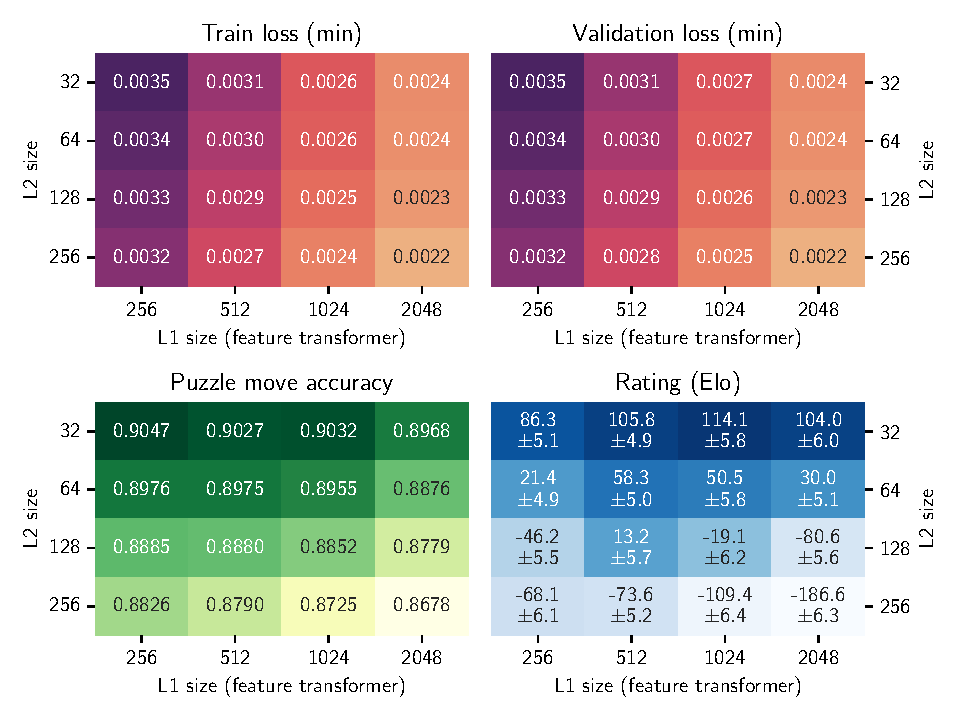
\includegraphics[width=0.93\textwidth]{../thesis/dynamic/output/baseline_heatmaps.pdf}}
\end{figure}
\end{frame}
